%%%%%%%%%%%%%%%%%%%%%%%%%%%
%%% PACKAGE DEFINITIONS %%%
%%%%%%%%%%%%%%%%%%%%%%%%%%%
\documentclass[10pt,english,handout,aspectradio=169]{beamer}


\usepackage{appendixnumberbeamer}
\usepackage{hyperref}

\usepackage{booktabs}
\usepackage[scale=2]{ccicons}

\usepackage{pgfplots}
\usepgfplotslibrary{dateplot}

\usepackage{xspace}
\newcommand{\themename}{\textbf{\textsc{metropolis}}\xspace}

\usepackage{pgfgantt}

\usepackage[newfloat,draft=false]{minted}

\definecolor{bg}{rgb}{0.96,0.96,0.98}


%%%%%%%%%%%%%
%%% EXTRA %%%
%%%%%%%%%%%%%
\usepackage{tcolorbox}
\tcbuselibrary{minted,skins,listings}
\newtcblisting{mytext}{
  listing engine=minted,
  colback=bg,
  listing only,
  minted style=bw,
  minted language=text,
  minted options={linenos=true,texcl=true,fontsize=\tiny},
  left=0.2mm,
  top=0cm,
  bottom=0cm,
  colframe=black!30,
  boxrule=0.1mm
}

%%%%%%%%%%%%%%%%%%%%%%%%%%%%%%%%%%%%%%%
%%% CUSTOMIZATION BEAMER-METROPOLIS %%%
%%%%%%%%%%%%%%%%%%%%%%%%%%%%%%%%%%%%%%%
\usetheme[progressbar=frametitle,block=fill,numbering=fraction]{metropolis}

\setbeamerfont{footnote}{size=\tiny}
\setbeamercolor{background canvas}{bg=white}

\AtBeginSection[]
{
   \begin{frame}
       \frametitle{Outline}
       \tableofcontents[currentsection,hideallsubsections]
%       \tableofcontents[currentsection]
   \end{frame}
}

%%%%%%%%%%%%%%
%%% DIAPOS %%%
%%%%%%%%%%%%%%
\title{Development of a virtualization framework with LXD}
\date{July 7, 2021}
\author{Òscar Pérez Castillo}
\institute{Universitat Politècnica de Catalunya}

\begin{document}

\maketitle

%%% TOC %%%
\begin{frame}{Table of contents}
  \setbeamertemplate{section in toc}[sections numbered]
  \tableofcontents[hideallsubsections]
\end{frame}

%%%%%%%%%%%%%%%%%%%%
%%% INTRODUCTION %%%
%%%%%%%%%%%%%%%%%%%%
\section{Introduction}
\begin{frame}{Introduction}
   Using Linux Containers, develop a framework on top of existing containerization solutions (LXC/LXD) improving:
   \begin{itemize}
       \item Containers organization
       \item Containers set up
       \item Containers distribution
   \end{itemize}
\end{frame}
\begin{frame}{Introduction}
    Developing a set of tools:
   \begin{itemize}
       \item lxce: command line tool
       \item lxce-admin: admin command line tool
       \item web application
   \end{itemize}
\end{frame}

%%%%%%%%%%%%%%%%%%%%%%
%%% GANTT DIAGRAM %%%%
%%%%%%%%%%%%%%%%%%%%%%
\section{Project organization}
\begin{frame}{Project organization}
\resizebox{10cm}{!}{\begin{ganttchart}[y unit title=0.4cm,
y unit chart=0.5cm,
vgrid,hgrid,
title height=1,
%today=25,%
%today offset=.5,%
%today label=Now,%
%bar/.style={draw,fill=cyan},
bar incomplete/.append style={fill=yellow!50},
bar height=0.7]{1}{24}

 % dies
 \gantttitle{Phases of the Project}{24} \\
 \gantttitle{2021}{24} \\
 \gantttitle{Feb}{4}
 \gantttitle{Mar}{5}
 \gantttitle{April}{5}
 \gantttitle{May}{5}
 \gantttitle{Jun}{5} \\
 
 % caixes elem0 .. elem9 
 % INTRODUCTION
 \ganttgroup[inline=false]{Introduction}{1}{2}\\
 \ganttbar[progress=100,bar/.style={draw,fill=cyan}]{Learn Javascript}{1}{1} \\
 \ganttbar[progress=100,bar/.style={draw,fill=cyan}]{Learn about containers}{2}{2} \\

 % LXCE
 \ganttgroup[inline=false]{lxce}{3}{16}\\
 \ganttbar[progress=100,bar/.style={draw,fill=red}]{v0.1}{3}{5} \\
 \ganttbar[progress=100,bar/.style={draw,fill=red}]{v0.2}{6}{8} \\
 \ganttbar[progress=100,bar/.style={draw,fill=red}]{v0.3}{9}{16} \\

 % LXCE-ADMIN
 \ganttgroup[inline=false]{lxce-admin}{14}{16}\\
 \ganttbar[progress=100,bar/.style={draw,fill=white}]{v0.1}{14}{16} \\

 % WEB ADMIN
 \ganttgroup[inline=false]{lxce-admin}{17}{20}\\
 \ganttbar[progress=90,bar/.style={draw,fill=black}]{Learn React/redux}{17}{19} \\
 \ganttbar[progress=10,bar/.style={draw,fill=black}]{Implement application}{20}{20} \\

 % relations
\ganttlink{elem2}{elem4}
\ganttlink{elem8}{elem10}


\end{ganttchart}
}
\end{frame}



%%%%%%%%%%%%%%%%%%%
%%% CONCEPTS %%%%%%
%%%%%%%%%%%%%%%%%%%
\section{Concepts}
\begin{frame}{Concepts}
    Project based on:
    \begin{itemize}
        \item Containers technology
        \item LXC
        \item LXD
    \end{itemize}
\end{frame}
\begin{frame}{Concepts: Containers}
Virtualization vs Containers
\begin{figure}
    \centering
    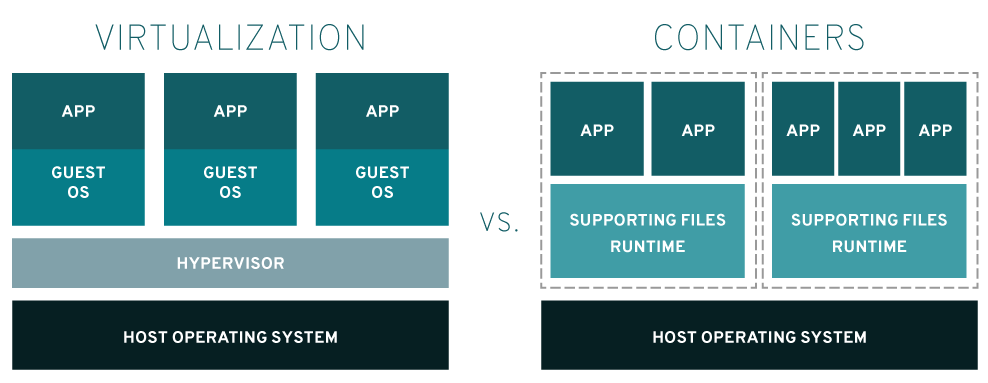
\includegraphics[width=\textwidth,height=\textheight,keepaspectratio]{img/02-state-virtualization-vs-containers} 
    \caption{ref: \href{https://www.redhat.com/en/topics/containers/whats-a-linux-container}{link}}
\end{figure}
\end{frame}
\begin{frame}{Concepts: Containers}
Abstracion created by the Linux Kernel:
\begin{itemize}
    \item Namespaces
    \item Cgroups
\end{itemize}
which provides:
\begin{itemize}
    \item Lightweight solution
    \item Isolation and control of resources
\end{itemize}
\end{frame}
\begin{frame}{Concepts: LXC}
\begin{itemize}
    \item C library (liblxc)
    \item Programming language bindings
    \item Tools for controlling containers
    \item Linux Distribution templates
\end{itemize}
    
\end{frame}
\begin{frame}{Concepts: LXD}
\begin{itemize}
    \item Build on top of LXC
    \item REST API
    \item New command line tool "lxc"
    \item Integration with containers services and other advanced features
\end{itemize}
    
\end{frame}
\begin{frame}[fragile]{Concepts: LXD}
Examples:
\begin{minted}[bgcolor=bg,breaklines,fontsize=\small,style=vs]{bash}
# Launch container
lxc launch ubuntu:20.04 box

# Launch a bash inside container
lxc exec box bash

# Add mapped proxy to the container
lxc config device add box testport80 listen=tcp:0.0.0.0:80 connect=tcp:127.0.0.1:80

# Share host folder with container
lxc config device add box device www disk source=/www datapath=/var/www/html
\end{minted}
    
\end{frame}

%%%%%%%%%%%%%%%%%%%
%%% DEVELOPMENT %%%
%%%%%%%%%%%%%%%%%%%
\section{Development}
\begin{frame}{Development}
Objective to develop a framework:
   \begin{itemize}
       \item Improve existing "lxc" command line tool - lxce
       \item Develop an admin tool - lxce-admin
       \item Develop a visual alternative to command line tool - web-admin
   \end{itemize} 
\end{frame}
%%% DEVELOPMENT-LXCE %%%
\begin{frame}{Development: lxce}
    \textbf{lxce} command line tool:
    \begin{itemize}
        \item Manage containers by configuration files.
        \item Organize containers by ``domains''.
        \item Organize containers by aliases.
        \item Configure proxies and shared folders by a configuration file.
        \item Generate SSH and VNC configuration files to be distributed.
    \end{itemize}
\end{frame}
\begin{frame}{Development: lxce}
Architecture:
\begin{figure}
    \centering
    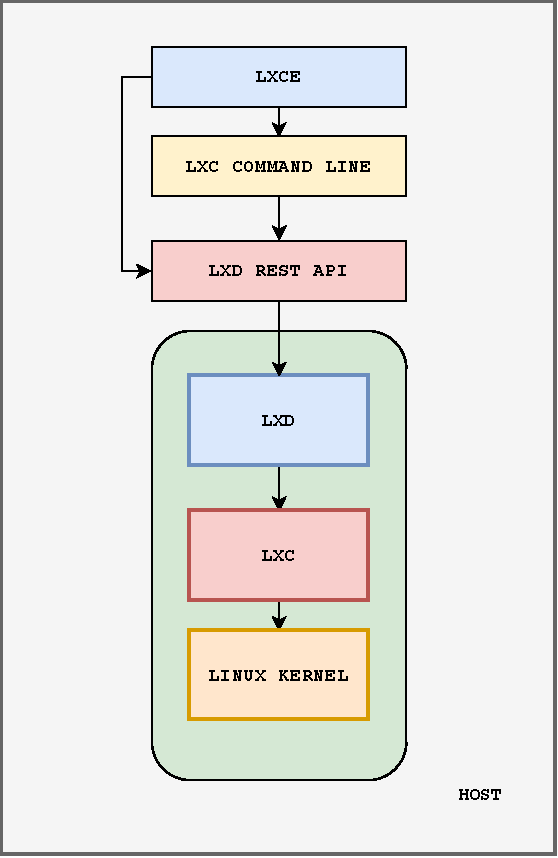
\includegraphics[scale=0.5]{img/lxce-diagram} 
\end{figure}
\end{frame}
\begin{frame}{Development: lxce}
Commands:
\begin{itemize}
    \item lxce init
    \item lxce alias
    \item lxce delete
    \item lxce launch
    \item lxce list
    \item lxce pass
    \item lxce proxy
    \item lxce rebase
    \item lxce show
    \item lxce start
    \item lxce stop
    \item lxce uninstall
\end{itemize}
\end{frame}
\begin{frame}[fragile]{Development: lxce}
Configuration files:
\begin{minted}[bgcolor=bg,breaklines,fontsize=\tiny,style=vs]{text}
/etc/lxce
|--- container.conf.d
|   |--- default
|   |   '--- voiceless-blue
|   '--- derecho
|       '--- relieved-beige
|--- container_default.conf
|--- lxce.conf
|--- remmina
|   |--- default
|   |   '--- oscar-vm.default.voiceless-blue.remmina
|   '--- derecho
|       '--- oscar-vm.derecho.relieved-beige.remmina
'--- ssh
    |--- default
    |   '--- voiceless-blue.conf
    '--- derecho
        '--- relieved-beige.conf
\end{minted}
\end{frame}
\begin{frame}[fragile]{Development: lxce}
Default configuration file:
\begin{minted}[bgcolor=bg,breaklines,fontsize=\tiny]{json}
{
  "name": "",
  "alias": "",
  "user": "",
  "id_domain": 0,
  "id_container": 0,
  
  "domain": "default",
  "base": "ubuntu:20.04",
  "userData": "/datasdd",
  
  "proxies": [
    {
      "name": "ssh",
      "type": "tcp",
      "listen": "0.0.0.0",
      "port": 22
    },
    {
      "name": "test",
      "type": "tcp",
      "listen": "0.0.0.0",
      "port": 3000
    }
  ],
}
\end{minted}
%%% DEMO ???? %%%
    
\end{frame}
%%% DEVELOPMENT-LXCE-ADMIN %%%
\begin{frame}{Development: lxce-admin}
    \textbf{lxce-admin} command line tool:
    \begin{itemize}
        \item Complete view of all container across different hosts
        \item Access to SSH and VNC configuration files
        \item VNC clients integrated
        \item Compute passwords for each container
    \end{itemize}
\end{frame}
\begin{frame}{Development: lxce-admin}
Architecture:
\begin{figure}
    \centering
    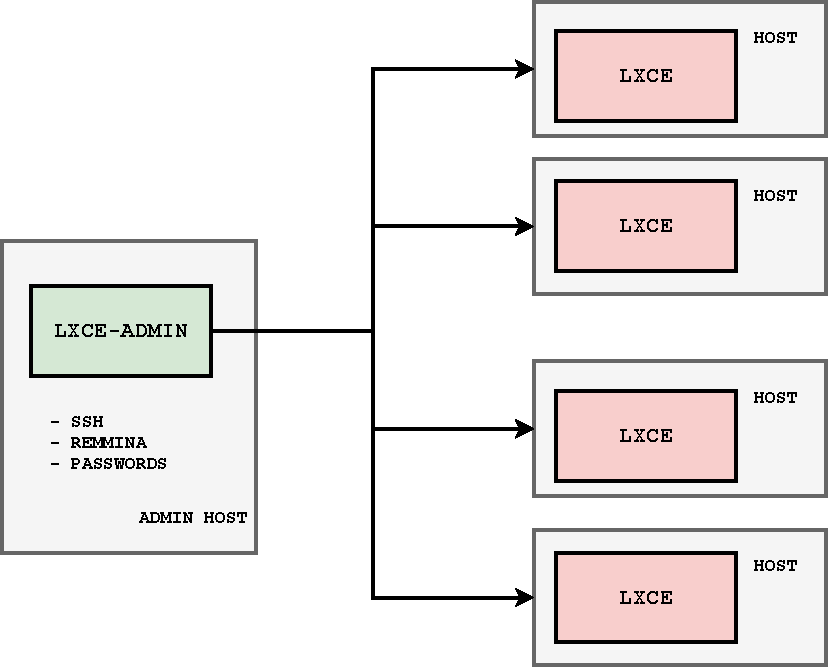
\includegraphics[scale=0.5]{img/lxce-admin-diagram.pdf} 
\end{figure}
\end{frame}
\begin{frame}{Development: lxce-admin}
Commands:
\begin{itemize}
    \item lxce-admin config add
    \item lxce-admin config list
    \item lxce-admin config remove
    \item lxce-admin config update
    \item lxce-admin pass
    \item lxce-admin remmina
    \item lxce-admin vnc
\end{itemize}
\end{frame}
%%% DEVELOPMENT-WEB-ADMIN %%%
\begin{frame}{Development: web-admin}
    \textbf{web admin} React web application:
    \begin{itemize}
        \item Visualize all current containers from each host
        \item Served along an API for each host
        \item Possibility to be extended
    \end{itemize}
\end{frame}
\begin{frame}{Development: web-admin}
Architecture:
\begin{figure}
    \centering
    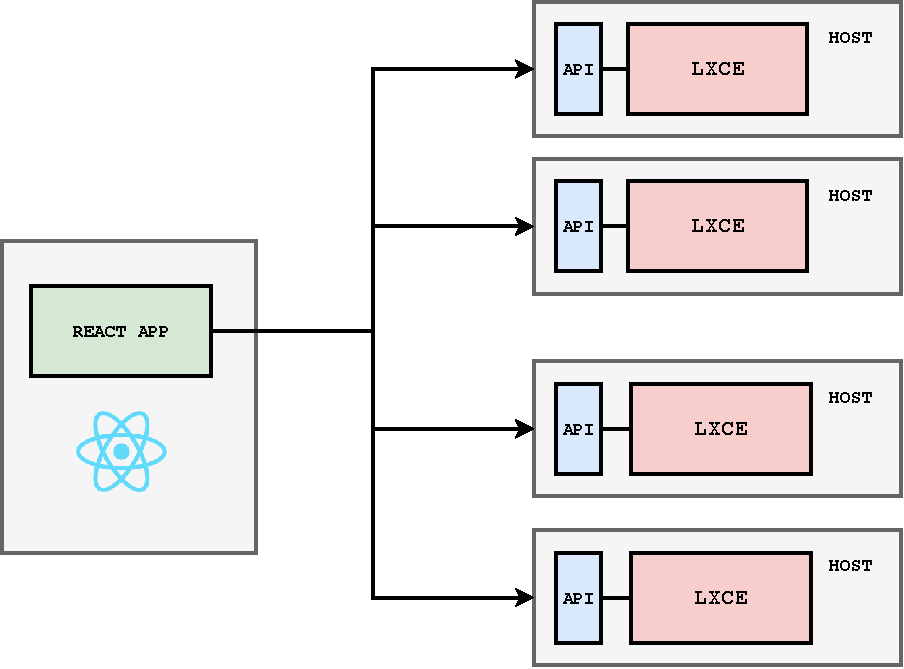
\includegraphics[scale=0.5]{img/web-admin-diagram.pdf} 
\end{figure}
\end{frame}

%%%%%%%%%%%%%%%%%%%
%%% FUTURE-WORK %%%
%%%%%%%%%%%%%%%%%%%
\section{Future work}
\begin{frame}{Future work}
Possible improvements:
    \begin{itemize}
        \item Add nginx and certificates functionality
        \item Extend API to provide more functionalities
    \end{itemize}
\end{frame}

%%%%%%%%%%%%%%%%%%
%%% CONCLUSION %%%
%%%%%%%%%%%%%%%%%%
\section{Conclusion}
\begin{frame}{Conclusion}
Learnt:
   \begin{itemize}
       \item Javascript/Typescript
       \item Containers 
       \item Web development
       \item Systems administration
   \end{itemize} 
\end{frame}

\begin{frame}[standout]
Thanks!
\end{frame}



%%% DEMO ??? %%%

\end{document}
